\documentclass{article}
\usepackage[utf8]{inputenc}
\usepackage{braket}
\usepackage{amsmath}
\usepackage{graphicx}
\usepackage{float}
\usepackage{hyperref}
\usepackage{caption}
\usepackage{subcaption}
\usepackage{derivative}

\usepackage{geometry}
\geometry{
    a4paper,
    total={170mm,257mm},
    left=20mm,
    top=20mm,
}

\graphicspath{ {../plots} }

\title{Simulating reaction of Ne* + OCS collision}
\author{Marcin Welter}
\date{Winter semester 2024/2025}

\newcommand{\centered}[1]{\begin{tabular}{l} #1 \end{tabular}}
\newcommand{\cmg}{\frac{\text{cm}^3}{\text{s}}}
\newcommand{\ak}{\hspace{50pt}}

\newcommand{\doubleImage}[2]{
    \begin{figure}[H]
        \centering
        \begin{subfigure}{.49\linewidth}
            \centering
            \includegraphics[width=\linewidth]{#1}
        \end{subfigure}
        \begin{subfigure}{.49\linewidth}
            \centering
            \includegraphics[width=\linewidth]{#2}
        \end{subfigure}
    \end{figure}
}

\newcommand{\doubleImageCaption}[5]{
    \begin{figure}[H]
        \centering
        \begin{subfigure}{.49\linewidth}
            \centering
            \includegraphics[width=\linewidth]{#1}
            \caption{#2}
        \end{subfigure}
        \begin{subfigure}{.49\linewidth}
            \centering
            \includegraphics[width=\linewidth]{#3}
            \caption{#4}
        \end{subfigure}
        \caption{#5}
    \end{figure}
}

\begin{document}
\maketitle

\section{Improved potential interpolations}
    Potential is now fitted to the force field instead of interpolation, because of smoothness issues.
    Gamma potentials now have correct vanishing derivatives for angles $0$ and $\pi$.

    \doubleImageCaption{potential.pdf}{Data}{potential_interp.pdf}{Fitted}{Fitting of intermolecular potential}
    
    \doubleImageCaption{xpi_gamma.pdf}{Data}{xpi_gamma_interp.pdf}{Interpolated}{Interpolation of $X\Pi$ gamma potential}
    
    \doubleImageCaption{bsigma_gamma.pdf}{Data}{bsigma_gamma_interp.pdf}{Interpolated}{Interpolation of $B\Sigma$ gamma potential}

    \doubleImageCaption{api_gamma.pdf}{Data}{api_gamma_interp.pdf}{Interpolated}{Interpolation of $A\Pi$ gamma potential}

\section{Truth tests for coriolis effect}
    Comparison of the ground state of the system defined by the space-fixed Hamiltonian
    \begin{equation}
        \hat{H} = -\frac{1}{2\mu} \pdv*[order=2]{}{R} + \frac{\hat{L}^2}{2 \mu R^2} + V(R, \theta),
    \end{equation}
    with our system in body-fixed frame for which we make rotational constant $B = 0$ and the Hamiltonian is
    \begin{equation}
        \hat{H} = -\frac{1}{2\mu} \pdv*[order=2]{}{R} + \frac{(\hat{J} - \hat{j})^2}{2 \mu R^2} + V(R, \theta).
    \end{equation}

    The conserved quantities for the first system is the angular momentum projection number $m_l$,
    in case of the body-fixed frame the conserved quantity is the total angular momentum $J$.

    In the case of harmonic oscillator potential
    \begin{equation}
        V(r, \theta) = \frac{\mu \omega^2}{2} (r - r_0)^2.
    \end{equation}

    The calculated ground state of the space-fixed Hamiltonian is then $\omega$ for $m = 0$.
    For the body-fixed Hamiltonian the calculated ground state for $J = 2$ is also $\omega$ with 
    coriolis effect and $1.15\omega$ if we neglect coriolis effect.

    \begin{figure}[H]
        \centering
        \begin{subfigure}{.4\linewidth}
            \centering
            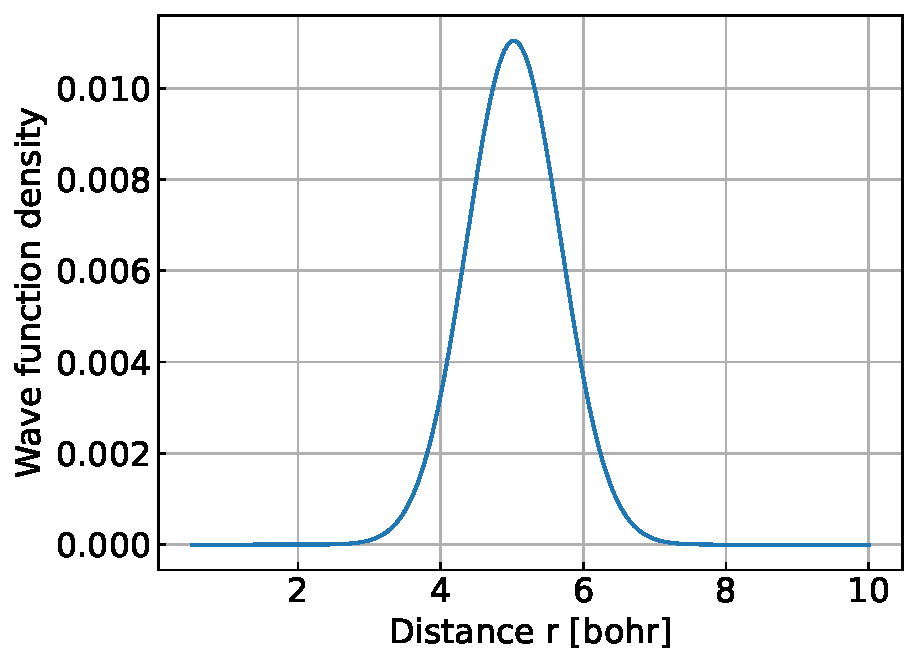
\includegraphics[width=\linewidth]{harmonic_iso_distance.pdf}
        \end{subfigure}
        \begin{subfigure}{.4\linewidth}
            \centering
            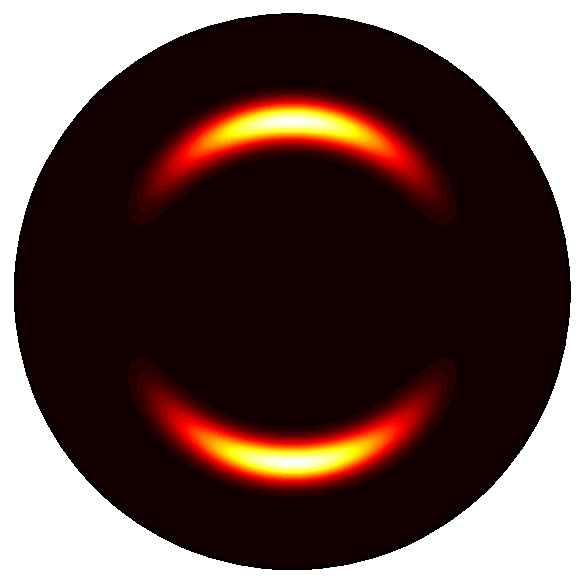
\includegraphics[width=\linewidth]{harmonic_iso_wave.pdf}
        \end{subfigure}
        \begin{subfigure}{.4\linewidth}
            \centering
            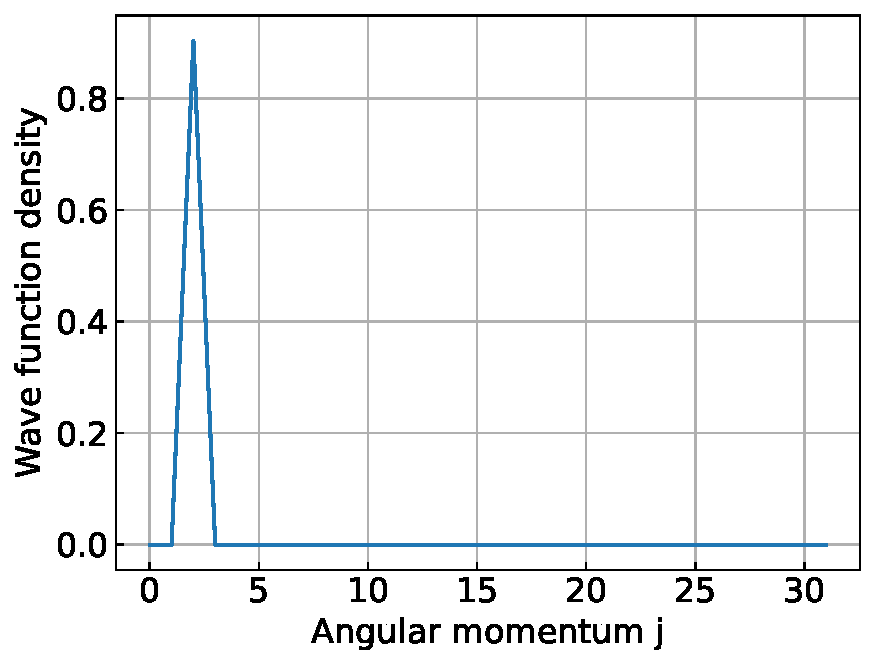
\includegraphics[width=\linewidth]{harmonic_iso_angular.pdf}
        \end{subfigure}
        \begin{subfigure}{.4\linewidth}
            \centering
            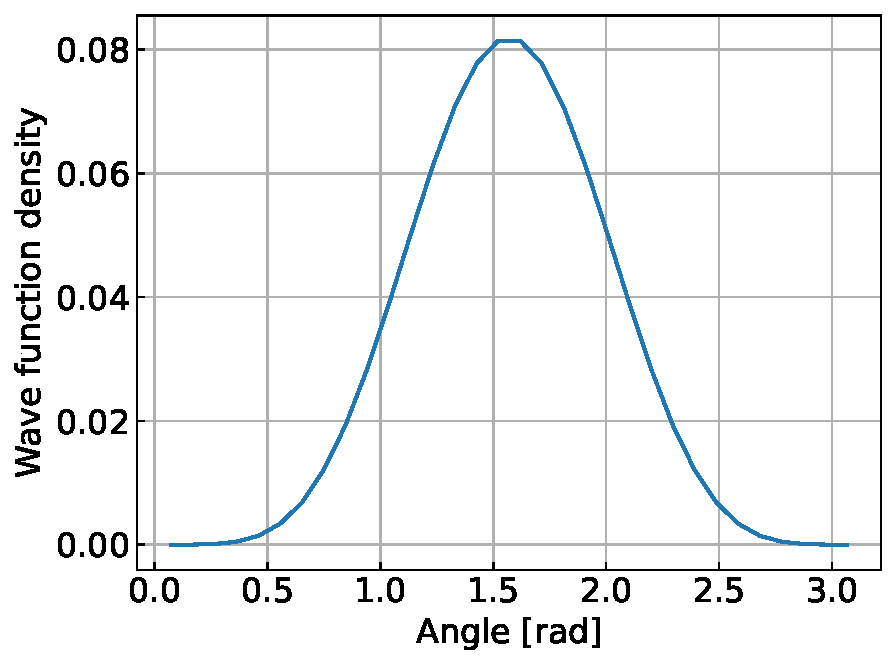
\includegraphics[width=\linewidth]{harmonic_iso_polar.pdf}
        \end{subfigure}
        \caption{Wave function calculated ground state for $J = 2$ without coriolis effect.}
    \end{figure}

    \begin{figure}[H]
        \centering
        \begin{subfigure}{.4\linewidth}
            \centering
            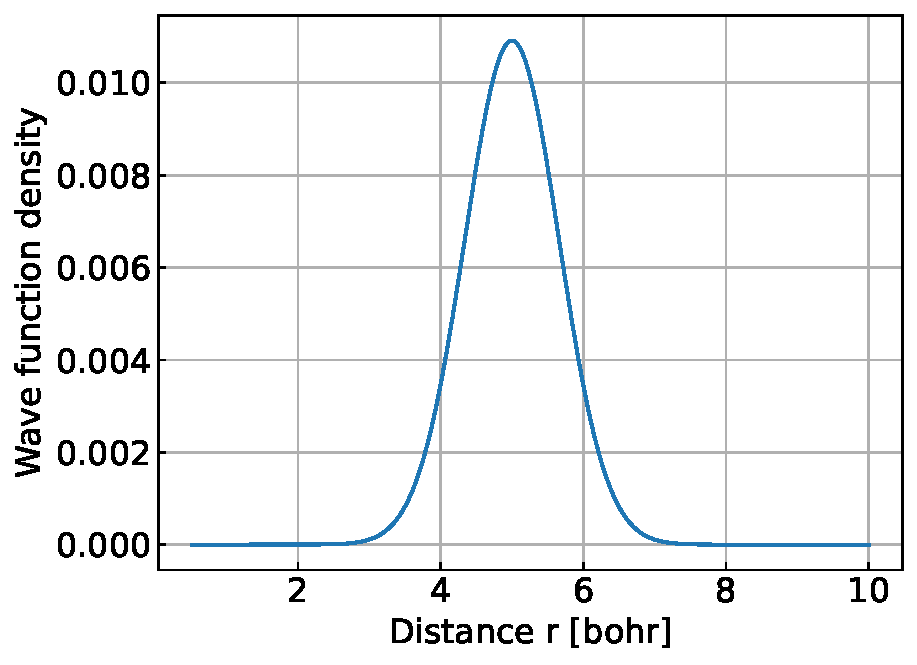
\includegraphics[width=\linewidth]{harmonic_iso_coriolis_distance.pdf}
        \end{subfigure}
        \begin{subfigure}{.4\linewidth}
            \centering
            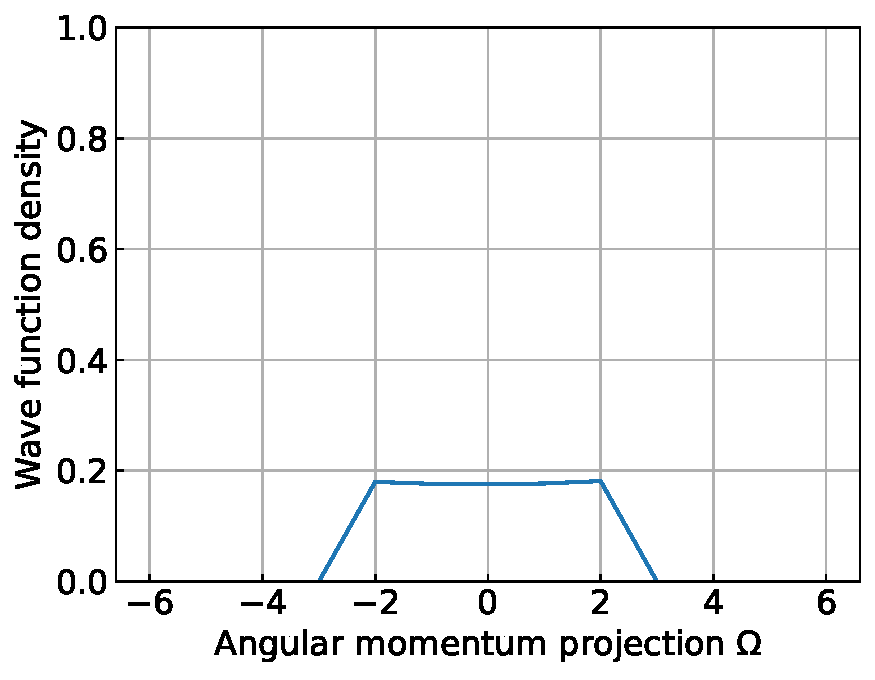
\includegraphics[width=\linewidth]{harmonic_iso_coriolis_omega.pdf}
        \end{subfigure}     
        \begin{subfigure}{.4\linewidth}
            \centering
            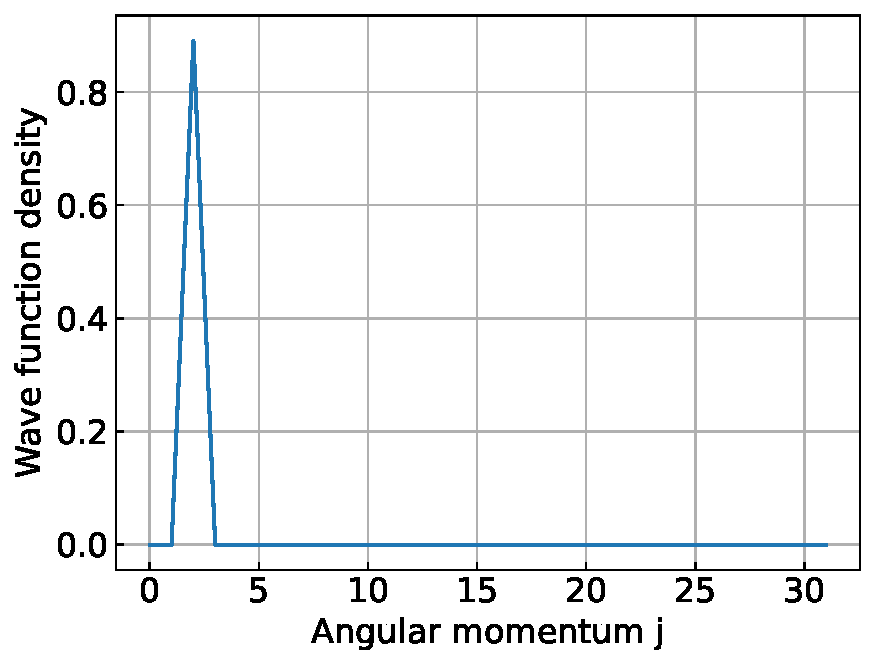
\includegraphics[width=\linewidth]{harmonic_iso_coriolis_angular.pdf}
        \end{subfigure}
        \begin{subfigure}{.4\linewidth}
            \centering
            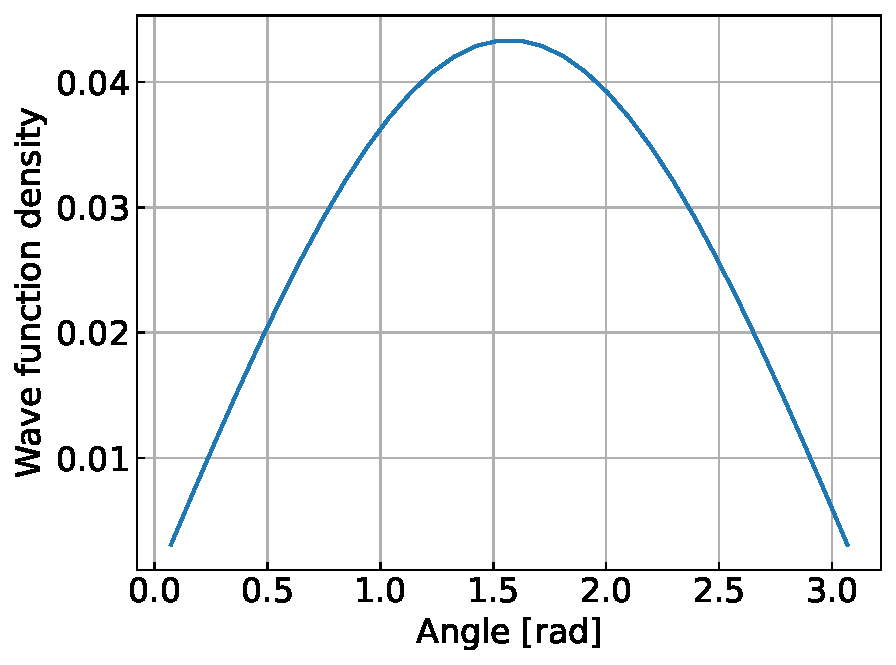
\includegraphics[width=\linewidth]{harmonic_iso_coriolis_polar.pdf}
        \end{subfigure}   
        \caption{Wave function calculated ground state for $J = 2$ with coriolis effect.}
    \end{figure}

    For potential of the form $V(r, \theta, \phi)$ the space-fixed Hamiltonian doesn't have any
    conserved angular numbers, however in body-fixed frame we have still $J$ conserved.
    It can be deduced that in the case of $B = 0$, $J$ gives additional infinite degeneracy,
    because of that for every conserved $J$ the ground state is $\omega$, 
    however only after the inclusion of coriolis effect.

\section{Reaction rate dependence on coriolis effect body-fixed projection cutoff}
    Animations of collisions with high $\Omega_\text{max}$ showed that the mixing of 
    total projection is up to $\Omega = 45$. However reaction rate calculations converge 
    for $\Omega_\text{max} = 2$, convergence test is shown below.

    \begin{figure}[H]
        \centering
        \begin{subfigure}{.4\linewidth}
            \centering
            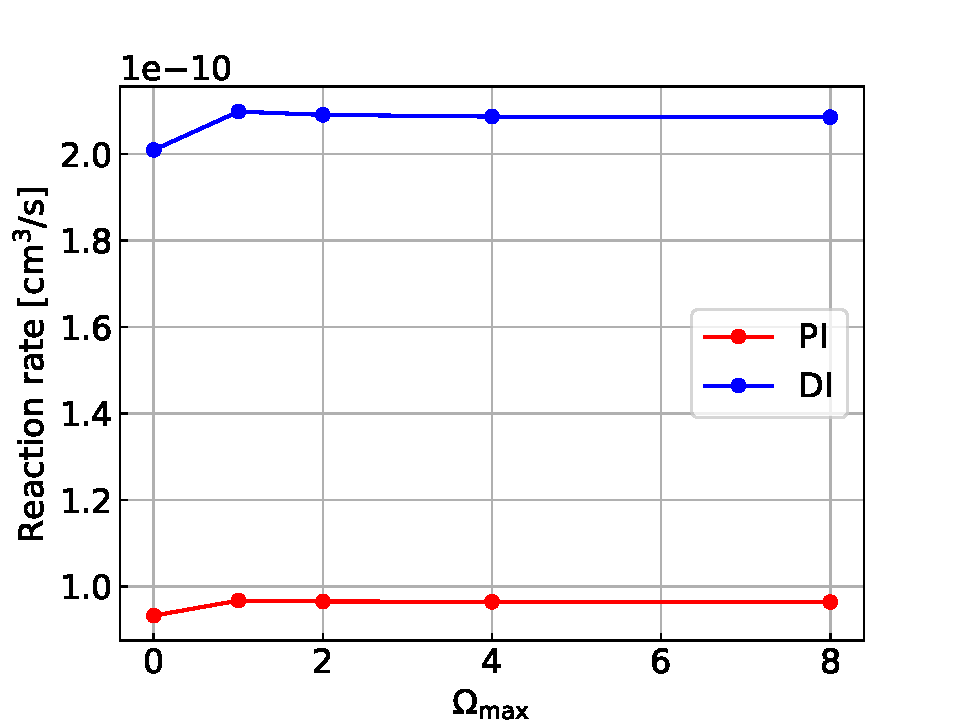
\includegraphics[width=\linewidth]{coriolis_rr_omega_maxes_0.pdf}
            \caption{Reaction rate for $j = 0$.}
        \end{subfigure}
        \begin{subfigure}{.4\linewidth}
            \centering
            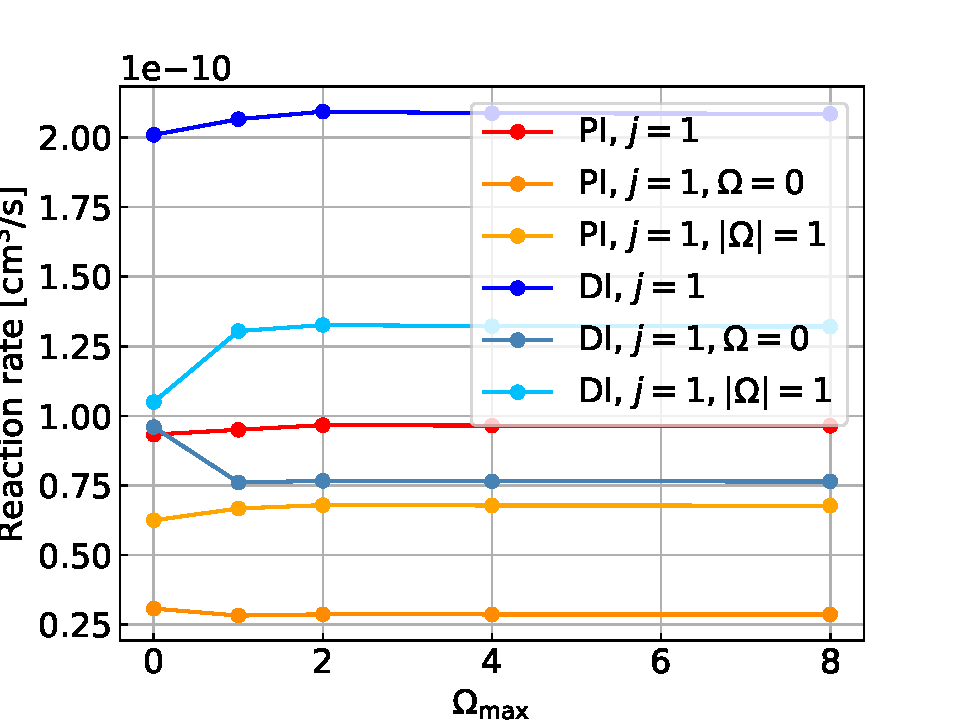
\includegraphics[width=\linewidth]{coriolis_rr_omega_maxes_1.pdf}
            \caption{Reaction rate for $j = 1$.}
        \end{subfigure}     
        \caption{Calculated reaction rates dependence on $\Omega_\text{max}$.}
    \end{figure}

    \begin{figure}[H]
        \centering
        \begin{subfigure}{.7\linewidth}
            \centering
            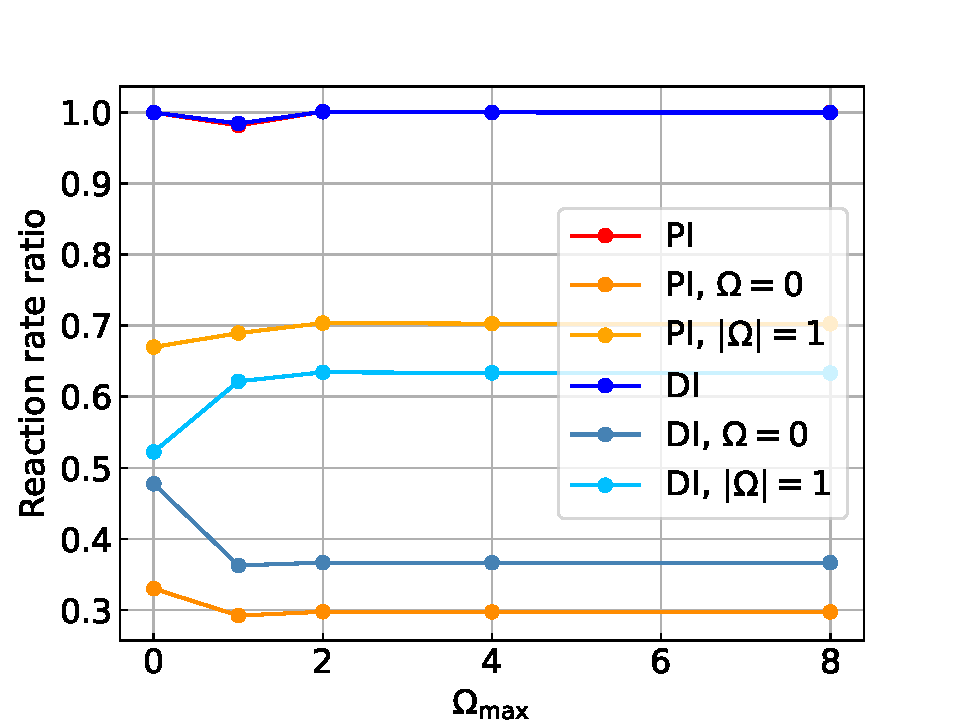
\includegraphics[width=\linewidth]{coriolis_rr_omega_maxes_ratio.pdf}
        \end{subfigure} 
        \caption{Calculated reaction rate ratio between $j = 1$ and $j = 0$, dependence on $\Omega_\text{max}$.}
    \end{figure}

    For the initial state $j = 1$ being the superposition of initial projections
    \begin{equation}
        \ket{\psi} = \frac{1}{\sqrt{3}} \left(e^{i\phi_{-1}}\ket{-1} + \ket{0} + e^{\phi_1}\ket{1}\right),
    \end{equation} 
    the reaction rate for different initial relative phases is shown below.

    \begin{figure}[H]
        \centering
        \begin{subfigure}{.4\linewidth}
            \centering
            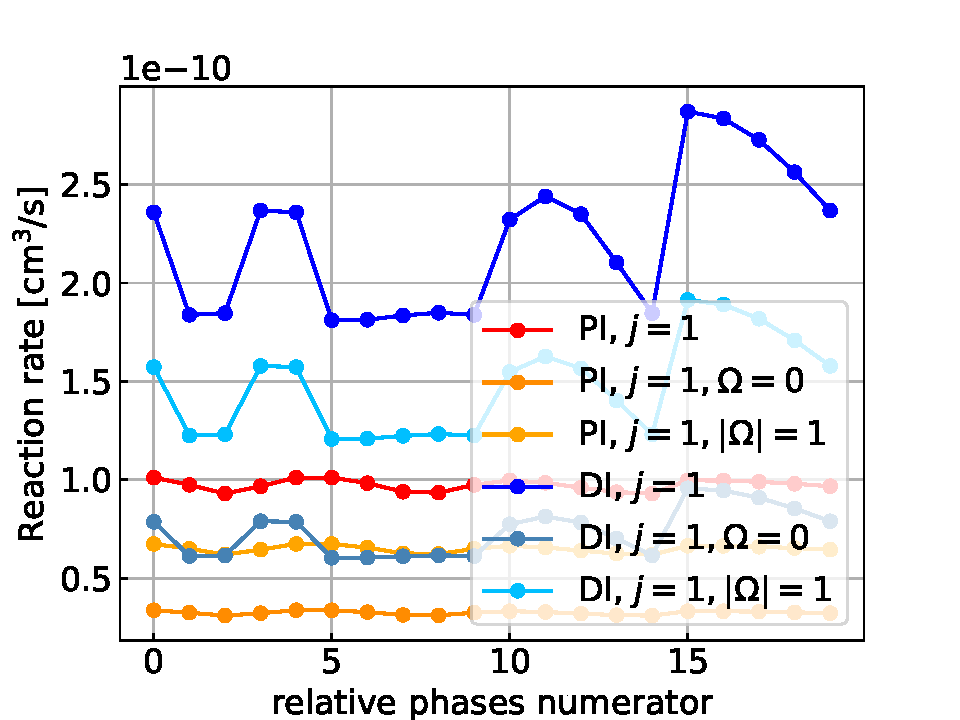
\includegraphics[width=\linewidth]{coriolis_reaction_rate_1_phases.pdf}
            \caption{Reaction rates for $j = 1$ for different phases.}
        \end{subfigure}
        \begin{subfigure}{.4\linewidth}
            \centering
            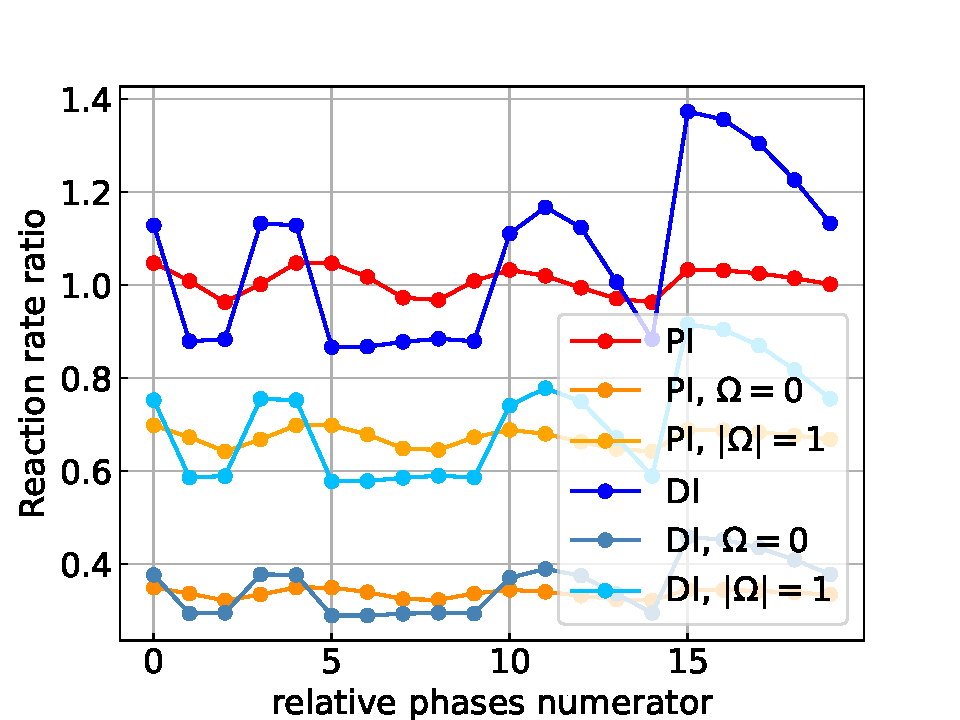
\includegraphics[width=\linewidth]{coriolis_reaction_rate_ratios_phases.pdf}
            \caption{Reaction rate for $j = 1$ for different phases}
        \end{subfigure}     
        \caption{Calculated reaction rates dependence for different phases.}
    \end{figure}

    \begin{figure}[H]
        \centering
        \begin{subfigure}{.7\linewidth}
            \centering
            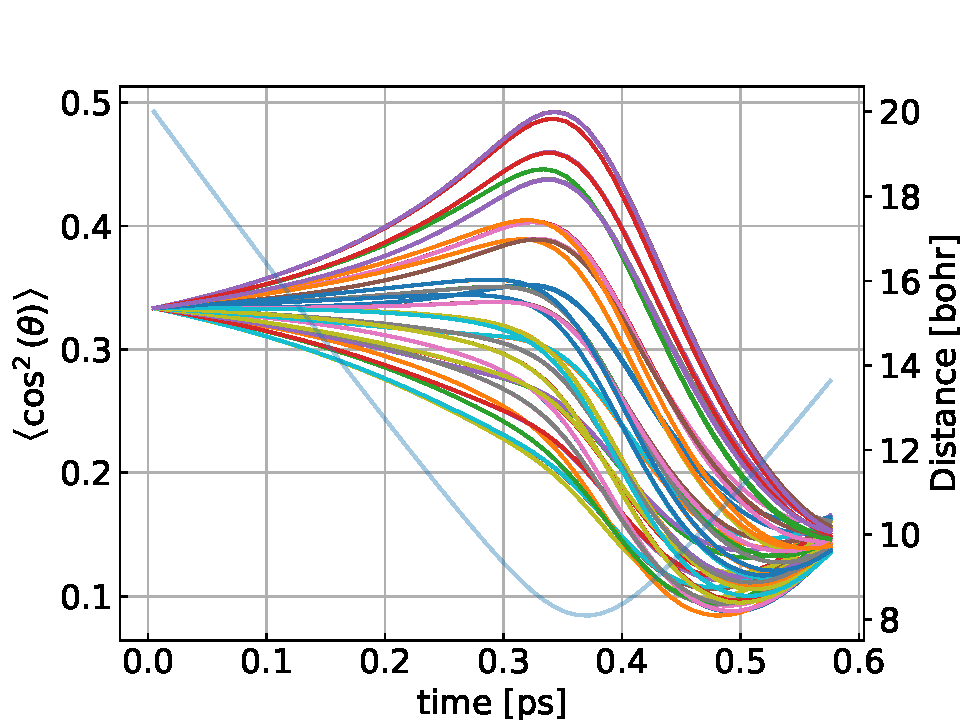
\includegraphics[width=\linewidth]{alignments_coriolis_phases.pdf}
        \end{subfigure} 
        \caption{Calculated alignments during the collision for different relative phases.}
    \end{figure}

    \section{Reaction rate ratios for force field scalings}
        Scaling the parameters of the force field did not change the reaction rate ratio
        from value of 1.

\end{document}